\chapter{Resultados e Discussão}
Neste capítulo discutimos os resultados obtidos durante a execução de nosso projeto. Na primeira parte apresentamos os gráficos da solução determinística da equação (\ref{ModeloDeterministicoEDO}). A dinâmica obtida a partir da solução numérica do sistema estocástico, apresentado na equação (\ref{EM}) é apresentada na segunda parte desse capítulo. 

\section{Resultados EDO}
Nessa seção exibimos graficamente, a dinâmica da solução analítica da EDO (\ref{eq1}). Assumimos o parâmetro de etiquetagem igual a uma unidade ($a = 1 $ e $ a = -1$). A solução apresentada na equação (\ref{eq1}) toma a forma:
\begin{eqnarray}\label{eq11111}
x(t) = \pm \frac{a}{\sqrt{(1- (1-\frac{a^{2}}{x_{0}^{2}}) e^{-4ta^{2}})}} , |x(0)| > a \\
x(t) = \pm \frac{a}{\sqrt{1+(\frac{a^{2}}{x_{0}^{2}} - 1)e^{-4ta^{2}}}} , |x(0)| < a
\end{eqnarray}
\begin{figure}[!htb]
\centering
\begin{minipage}[b]{0.9\linewidth}
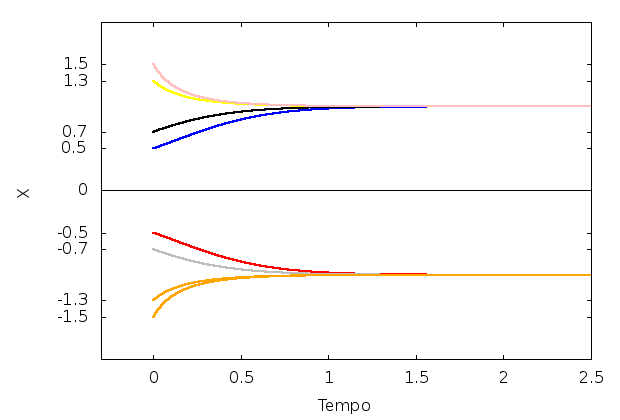
\includegraphics[width=\linewidth]{./img/analiseAssimptotica.png}
\caption{Solução analítica da EDO (\ref{ModeloDeterministicoEDO}).}
\label{fig0}
\end{minipage} \hfill
\end{figure}
Visualizamos $x(t)$ sob diversas condições iniciais, as quais são representadas pelas seguintes curvas: Cinza $x(0) = -0.5$,  verde $x(0) = -0.7$, vermelha $x(0) = -1.3$, laranja $x(0) = -1.5$, amarela $x(0) = 0.5$, azul $x(0) = 0.7$, preta $x(0) = 1.3$ e rosa $x(0) = 1.5$. Na figura (\ref{fig0}) apresentamos a dinâmica de $x_{0}$ como função do tempo de acordo com a condição inicial. Para $x(0)$ positivo, temos convergência para a solução de equilibrio assimptótico $\overline{x}_{+} = a$ e, convergência para $\overline{x}_{-} = -a$ em caso de $x(0)$ negativo. Uma característica que independe do estado inicial do sistema é seu decaimento para o regime estacionário. O parâmetro $a$, determina um tempo máximo para a meia-vida do regime dinâmico, dado como $\frac{1}{4a^{2}}$. Podemos observar que no caso de condições iniciais satisfazendo $x(0) > 0$, temos o limite assimptótico:
\begin{eqnarray}
\lim_{x \rightarrow +\infty} x(t) ,
\end{eqnarray}
e para o caso de condições iniciais satisfazendo $x(0) < 0$, temos o limite assimptótico:
\begin{eqnarray}
\lim_{x \rightarrow -\infty} x(t) .
\end{eqnarray}
Os gráficos confirmam que a vizinhança dos valores de $\overline{x}_{\pm}$ são condições de equilíbrio estável do sistema, conforme discutido no capítulo 3. Note que estamos tratando um sistema dissipativo, em que não ocorrem oscilações.

\section{Resultados EDE}
Nessa seção exibimos graficamente, a dinâmica da solução analítica da EDE (\ref{Cubo}). Assumimos o parâmetro de etiquetagem igual a uma unidade ($a = 1 $ e $ a = -1$). A solução apresentada na equação (\ref{Cubo}) toma a forma:
\begin{eqnarray}\label{eq11111222}
x_{n+1} = x_{n} - 2x_{n}(x_{n} - a)(x_{n} + a)h + \sigma N(0,1) \sqrt{h}
\end{eqnarray}
\begin{figure}[!htb]
\centering
\begin{minipage}[b]{0.9\linewidth}
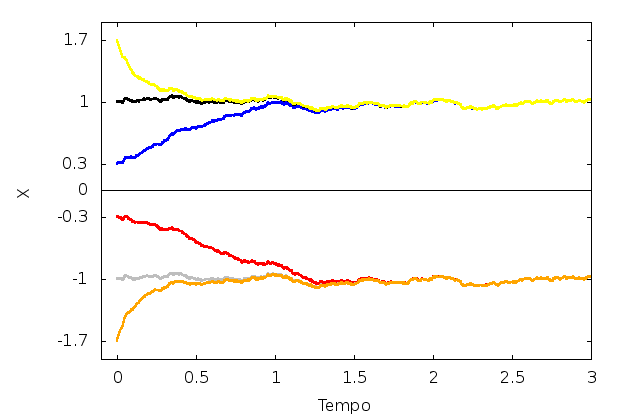
\includegraphics[width=\linewidth]{./img/analiseAssimptoticaEM.png}
\caption{Solução numérica da EDE (\ref{Cubo}).}
\label{fig0000}
\end{minipage} \hfill
\end{figure}
Visualizamos $x(t)$ sob diversas condições iniciais, as quais são representadas pelas seguintes curvas: amarela $x(0) = 1.7$, preta $x(0) = a$, azul $x(0) = 0.3$, vermelha $x(0) = -0.3$, cinza $x(0) = -a$ e laranja $x(0) = -1.7$. Uma característica que independe do estado inicial do sistema é seu decaimento para o regime estacionário. O parâmetro $a$, determina um tempo máximo para a meia-vida do regime dinâmico, dado como $\frac{1}{4a^{2}}$. Podemos observar que no caso de condições iniciais satisfazendo $x(0) > 0$, temos o limite assimptótico:
\begin{eqnarray}
\lim_{x \rightarrow +\infty} x(t) ,
\end{eqnarray}
e para o caso de condições iniciais satisfazendo $x(0) < 0$, temos o limite assimptótico:
\begin{eqnarray}
\lim_{x \rightarrow -\infty} x(t).
\end{eqnarray}

\section{Resultados EDE x EDO}
Nessa seção serão comparados os resultados da EDO com a EDE para diferentes valores de ruído.
Incluímos as trajetórias para $x(t)$ sob a condição inicial $x(0) = 0.7$. Assumindo o parâmetro de etiquetagem igual à unidade ($a=1$). Nós mostramos que valores da amplitude de ruído influenciam o comportamento do sistema em tempos assimptóticos como segue:

\begin{itemize}
\item[i)]   $\sigma = 0.1 \textrm{ , } x(t) \textrm{ \mbox{f}lutua em torno do valor de } \overline{x}_{+} = 1$;

\item[ii)]  $\sigma = 0.5\textrm{ , } x(t) \textrm{ \mbox{f}lutua em torno de } \overline{x}_{+} = 1$ 
por um certo intervalo e salta para a vizinhança de $\overline{x}_{-} = -1$ , flutuando nessa região;

\item[iii)] $\sigma = 2 \textrm{ , } x(t) \textrm{ \mbox{f}lutua em torno de } \overline{x}_{+} = 0$, desvio padrão da ordem de 1.
\end{itemize}

Agora serão exibidos os gráficos que plotamos a fim de facilitar a análise da solução da 
EDO com diferentes valores de ruído.

\begin{figure}[!htb]
\centering
\begin{minipage}[b]{0.55\linewidth}
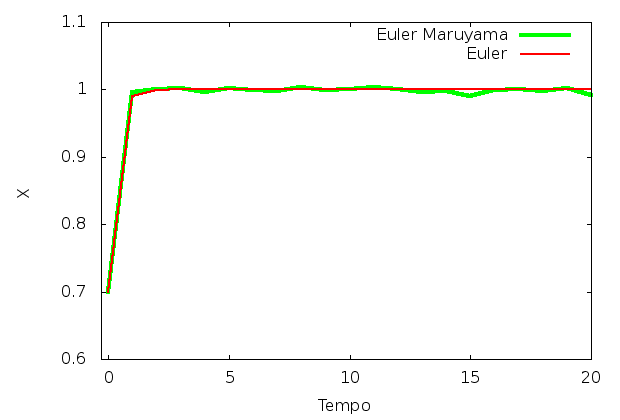
\includegraphics[width=\linewidth]{./img/Langevin_CI07_ruido001.png}
\caption{Onde $x(0) = 0.7 ; a = 1 ; \sigma = 0.01$}
\label{fig1}
\end{minipage} \hfill
\end{figure}

Na figura \ref{fig1} analisamos a dinâmica de $x$ para $\sigma = 0.01$ e condição inicial, $x(0) = 0.7$ para a 
equação ${dx} = -2x(x-a)(x+a)dt + \sigma N(0,1) \sqrt{dt}$ (\ref{Cubo}) utilizando o algorítmo de Euler-Maruyama, 
eq. $X_n = X_{n-1} + 2X_{n-1}(X_{n-1} - a)(X_{n-1} + a)h + \sigma N(0,1) \sqrt(h)$ (\ref{EM}).

Neste caso, verificamos que $x(t)$ é um processo estocástico cujos valores: $x(t_{0}, t_{1}, t_{2},...)$ para 
$t_{0} < t_{1} < t_{2}$, flutuam aleatóriamente em torno de dois valores de equilíbrio assimptótico da EDO (\ref{ModeloDeterministicoEDO}) $ \pm a$. Essa característica interessante se deve ao aumento do valor de $\sigma$." Antepenultimo da seção de resultados 4.

\begin{figure}[!htb]
\centering
\begin{minipage}[b]{0.55\linewidth}
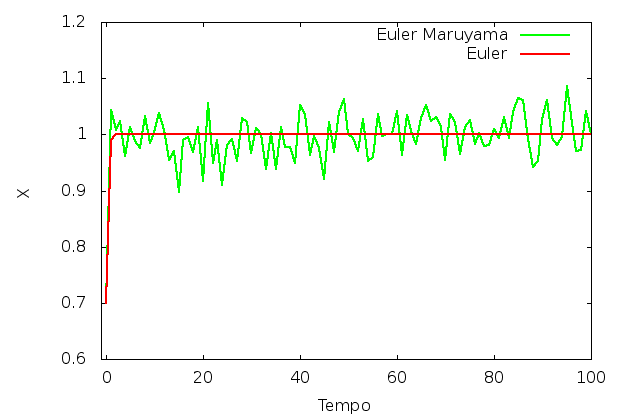
\includegraphics[width=\linewidth]{./img/Langevin_CI07_ruido01.png}
\caption{Onde $x(0) = 0.7 ; a = 1 ; \sigma = 0.1$}
\label{fig2}
\end{minipage} \hfill
\end{figure}

Na figura \ref{fig2} analisamos a dinâmica de $x$ para $\sigma = 0.1$ e condição inicial, $x(0) = 0.7$ para a 
equação ${dx} = -2x(x-a)(x+a)dt + \sigma N(0,1) \sqrt{dt}$ (\ref{Cubo}) utilizando o algorítmo de Euler-Maruyama, 
eq. $X_n = X_{n-1} + 2X_{n-1}(X_{n-1} - a)(X_{n-1} + a)h + \sigma N(0,1) \sqrt(h)$ (\ref{EM}).

Neste caso, verificamos que $x(t)$ é um processo estocástico cujos valores: $x(t_{0}, t_{1}, t_{2},...)$ para 
$t_{0} < t_{1} < t_{2}$, flutuam aleatóriamente em torno do valor assimptótico determinístico $x^{+}(+\infty) = 1$ correspondente à condição inicial assumida $x(0) = 0.7$, porém, esse valor de $\sigma$ consegue causar uma perturbação 
maior na solução.

\begin{figure}[!htb]
\centering
\begin{minipage}[b]{0.55\linewidth}
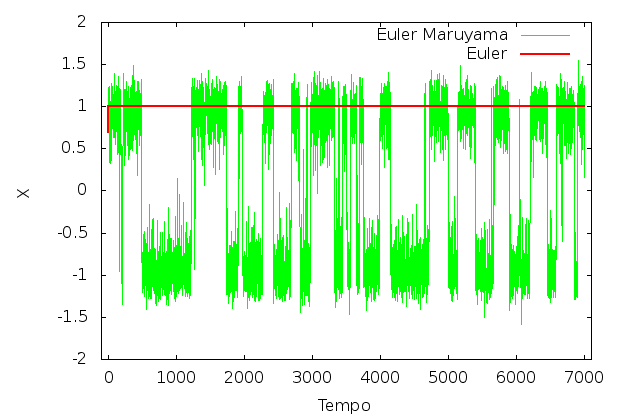
\includegraphics[width=\linewidth]{./img/Langevin_CI07_ruido05.png}
\caption{Onde $x(0) = 0.7 ; a = 1 ; \sigma = 0.5$}
\label{fig3}
\end{minipage} \hfill
\end{figure}

Na figura \ref{fig3} analisamos a dinâmica de $x$ para $\sigma = 0.5$ e condição inicial, $x(0) = 0.7$ para a eq. 
${dx} = -2x(x-a)(x+a)dt + \sigma N(0,1) \sqrt{dt}$ (\ref{Cubo}) utilizando o algorítmo de Euler-Maruyama: 
$X_n = X_{n-1} + 2X_{n-1}(X_{n-1} - a)(X_{n-1} + a)h + \sigma N(0,1) \sqrt(h)$ (\ref{EM}).

Neste caso, verificamos que $x(t)$ é um processo estocástico cujos valores: $x(t_{0}, t_{1}, t_{2},...)$ para 
$t_{0} < t_{1} < t_{2}$, flutuam aleatóriamente em torno de dois valores assimptóticos: o valor  $x^{+}(+\infty) = 1$ correspondente à condição inicial assumida $x(0) = 0.7$, e o valor $x^{-}(+\infty) = -1$, que representam os valores de a e -a, respectivamente, no caso determinístico. Essa característica interessante se deve ao aumento do valor de $\sigma$.

\begin{figure}[!htb]
\centering
\begin{minipage}[b]{0.55\linewidth}
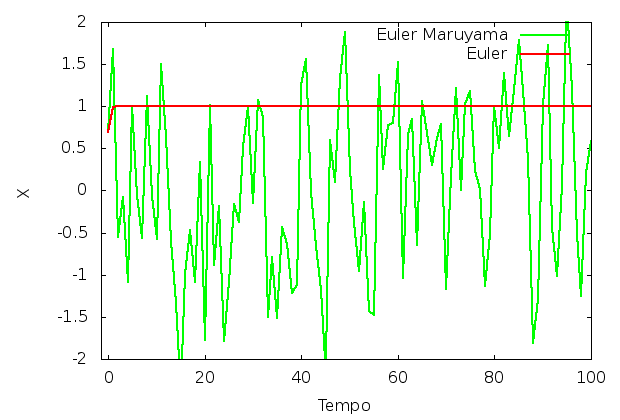
\includegraphics[width=\linewidth]{./img/Langevin_CI07_ruido2.png}
\caption{Onde $x(0) = 0.7 ; a = 1 ; \sigma = 2$}
\label{fig4}
\end{minipage} \hfill
\end{figure}

Na figura \ref{fig4} analisamos a dinâmica de ${x}$ para ${\sigma} = 2$ e condição inicial, $x(0) = 0.7$ para a eq. ${dx} = -2x(x-a)(x+a)dt + \sigma N(0,1) \sqrt{dt}$ (\ref{Cubo}) utilizando o algorítmo de Euler-Maruyama, 
eq. $X_n = X_{n-1} + 2X_{n-1}(X_{n-1} - a)(X_{n-1} + a)h + \sigma N(0,1) \sqrt(h)$ (\ref{EM}).

Neste caso, verificamos que $x(t)$ é um processo estocástico cujos valores: $x(t_{0}, t_{1}, t_{2},...)$ para 
$t_{0} < t_{1} < t_{2}$, flutuam aleatóriamente não apresentando um resultado tão interessante quanto o $\sigma = 0.5$.